\documentclass{standalone}
\usepackage{tikz}
\usepackage{ifthen}
\usepackage{pgfmath}


%\def\levelColor{{"red"}}

\def\color{{"redstyle","redstyle","redstyle","redstyle","redstyle","redstyle","bluestyle","bluestyle","bluestyle","redstyle","redstyle","bluestyle","bluestyle","redstyle","redstyle","bluestyle","bluestyle","redstyle","redstyle","bluestyle","bluestyle","redstyle","redstyle","redstyle","bluestyle","bluestyle","bluestyle","bluestyle","bluestyle","bluestyle","bluestyle"}}

\def\size{15} %size-1
\begin{document}
	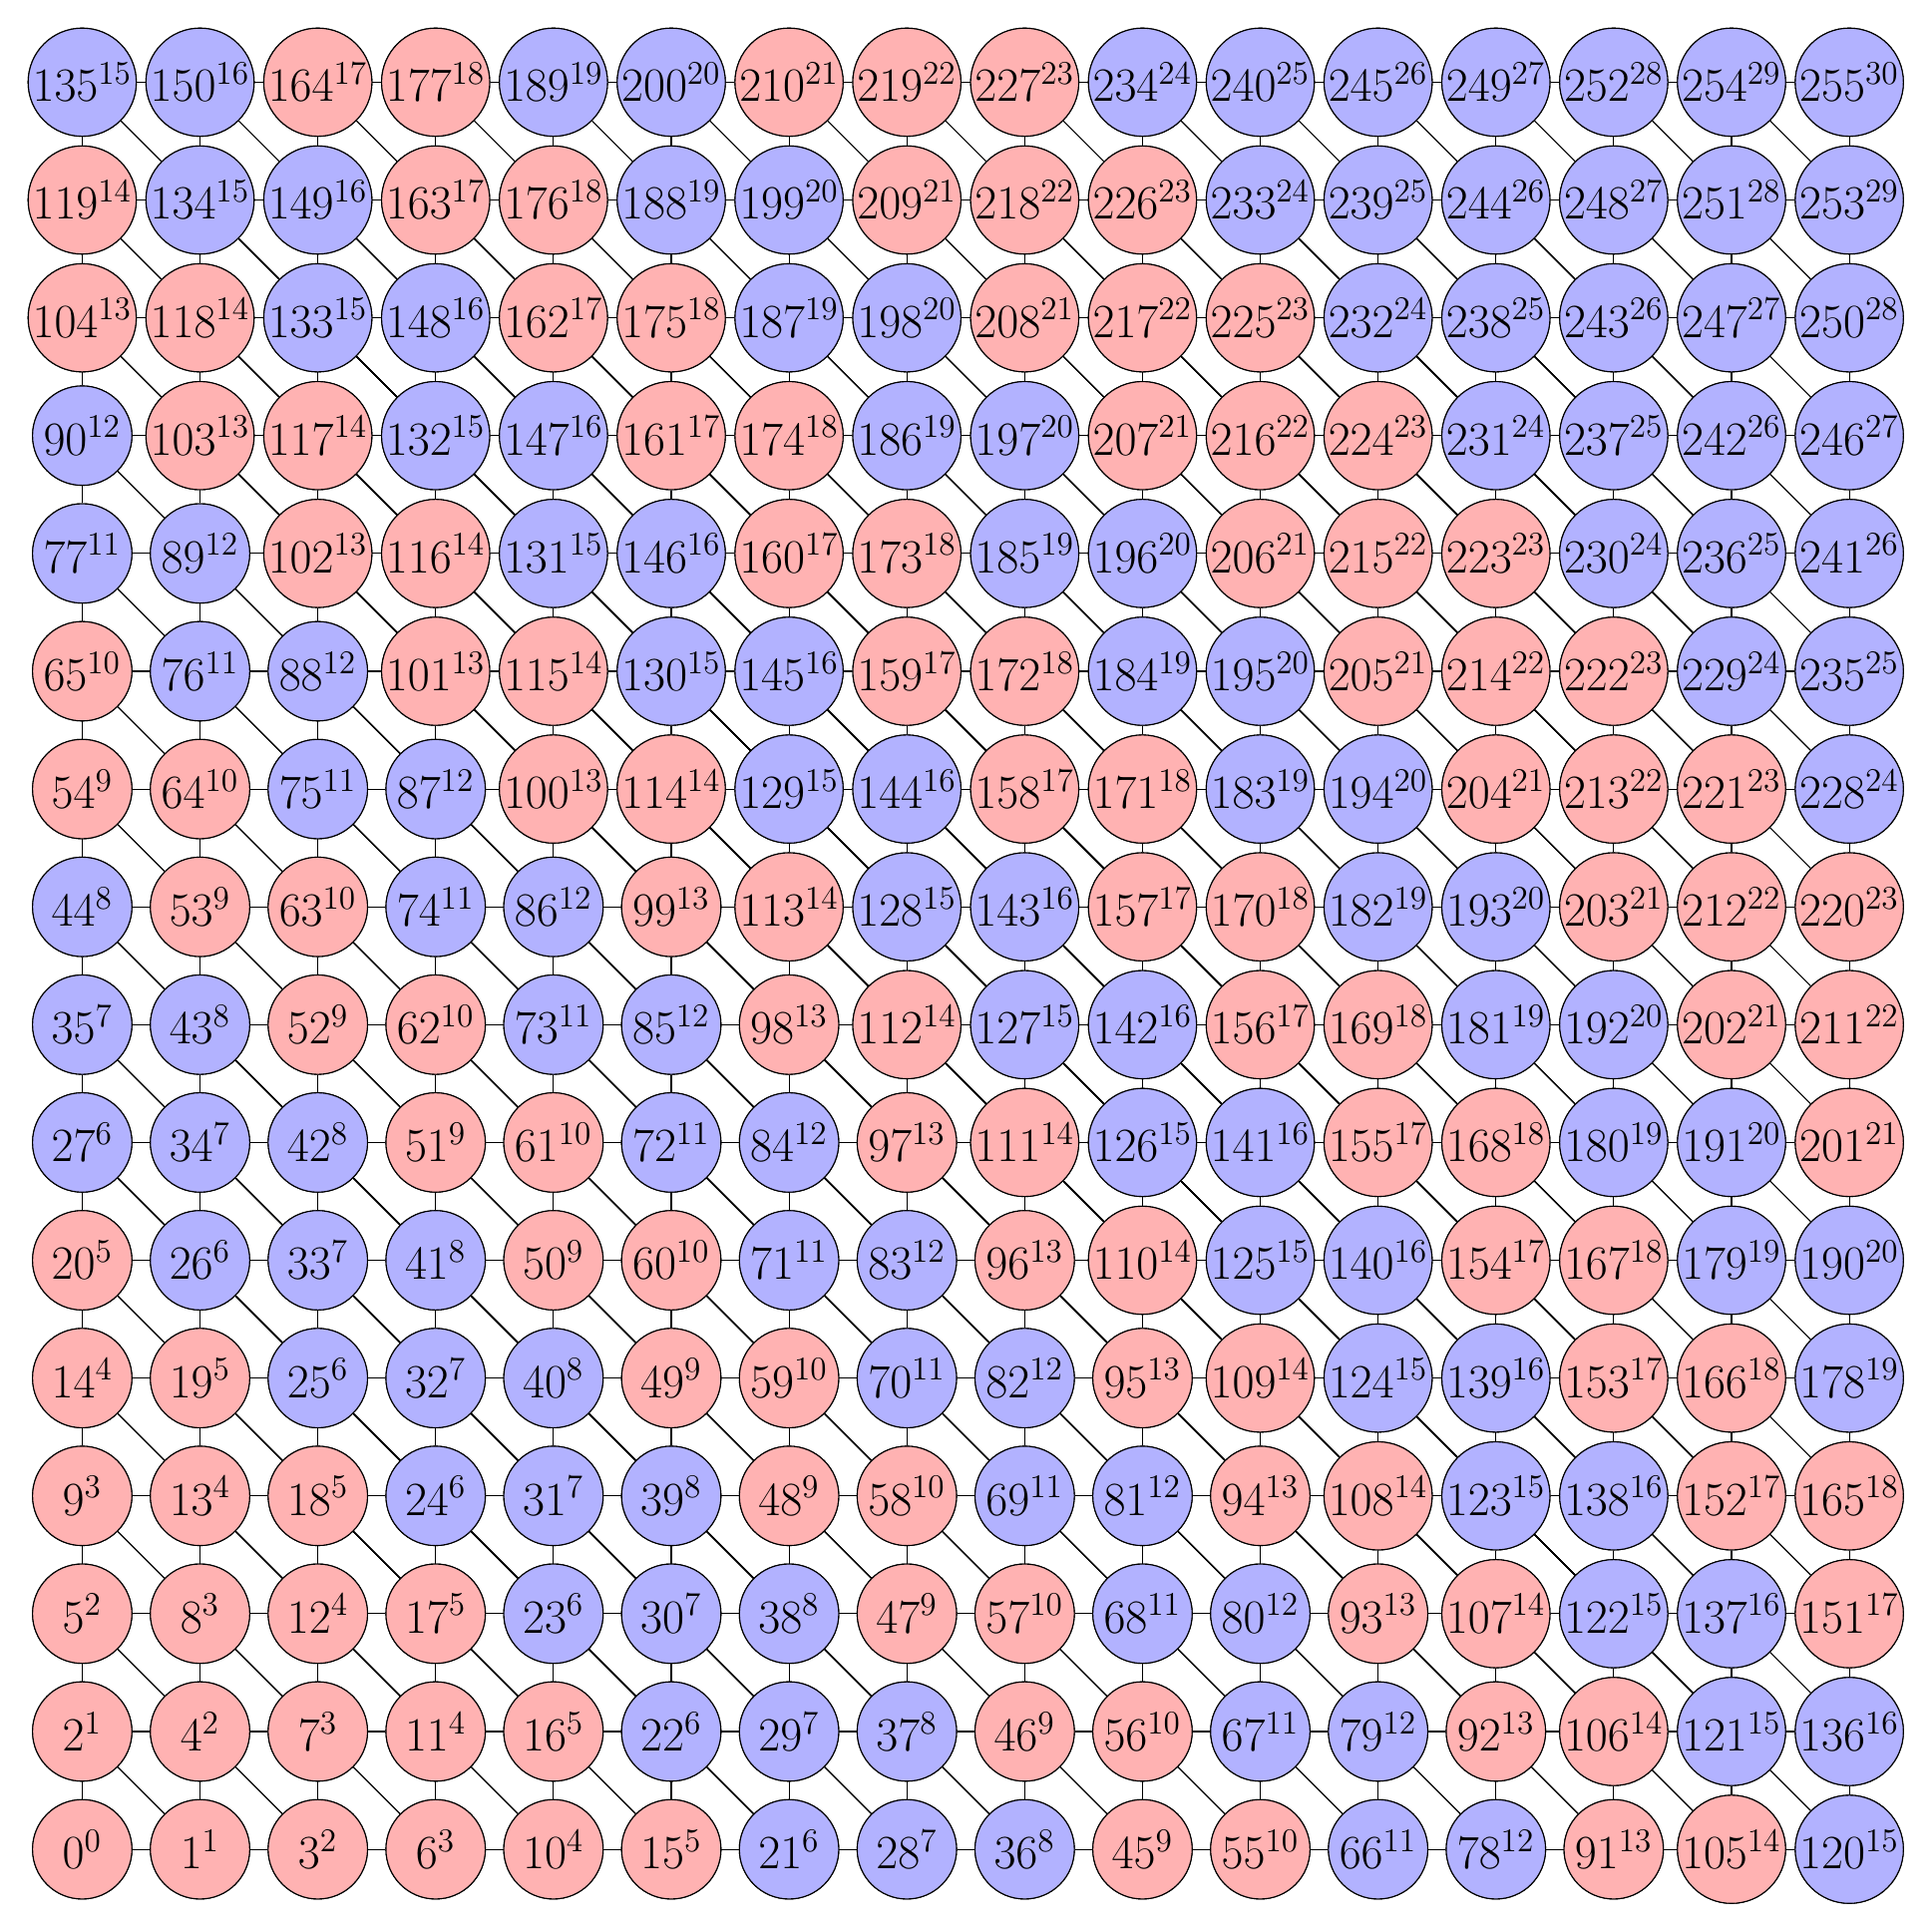
\begin{tikzpicture}[redstyle/.style={circle,draw,fill=red!30!white,minimum size=36, inner sep=0.2pt}, bluestyle/.style={circle,draw,fill=blue!30!white,minimum size=36, inner sep=0.2pt}]
	\foreach \x in {0,...,\size}
	\foreach \y in {0,...,\size} 
	{
		\pgfmathtruncatemacro{\sizepone}{\size+1 }
		\pgfmathtruncatemacro{\label}{\y*\sizepone + \x  }
		\pgfmathtruncatemacro{\labell}{(\y + \x)*(\y+\x+1)*0.5+\y  }
		\pgfmathtruncatemacro{\labelu}{((\size+1)*(\size+1)-1) - (((\size*2) - \y - \x)*((\size*2) - \y-\x + 1)*0.5+ \size-\y)  }
		\pgfmathtruncatemacro{\level}{\y + \x  }
		\pgfmathtruncatemacro{\yinv}{\size - \y }
	
		\pgfmathparse{\color[\level]}
		\edef\currCOLOR{\pgfmathresult}
	%	\edef\currColor{\pgfmathresult}
		\node[\currCOLOR]  (\label) at (1.5*\x,1.5*\y) { \ifthenelse{\x > \yinv} {\LARGE{\labelu$^{\large{\level}}$}} {\LARGE{\labell$^{\large{\level}}$}}} ;
		;}
	
	\foreach \x in {0,...,\size}
	{
		\pgfmathtruncatemacro{\sizemone}{\size-1 }
		\pgfmathtruncatemacro{\sizepone}{\size+1 }
		\foreach \y [count=\yi] in {0,...,\sizemone}  
		{
			\pgfmathtruncatemacro{\labelone}{\y*\sizepone + \x  }
			\pgfmathtruncatemacro{\labeltwo}{\yi*\sizepone + \x  }
			\pgfmathtruncatemacro{\labelthree}{\x*\sizepone + \y  }
			\pgfmathtruncatemacro{\labelfour}{\x*\sizepone + \yi  }
			\draw (\labelone)--(\labeltwo) (\labelthree)--(\labelfour) ;
			\draw (\labelone)-- (\labelthree);
		}
	}
	
	\foreach \x in {0,...,\size}
	\foreach \y in {0,...,\size} 
	{
		\pgfmathtruncatemacro{\sizepone}{\size+1 }
		\pgfmathtruncatemacro{\label}{\y*\sizepone + \x  }
		\pgfmathtruncatemacro{\labell}{(\y + \x)*(\y+\x+1)*0.5+\y  }
		\pgfmathtruncatemacro{\labelu}{((\size+1)*(\size+1)-1) - (((\size*2) - \y - \x)*((\size*2) - \y-\x + 1)*0.5+ \size-\y)  }
		\pgfmathtruncatemacro{\level}{\y + \x  }
		\pgfmathtruncatemacro{\yinv}{\size - \y }
		
		\pgfmathparse{\color[\level]}
		\edef\currCOLOR{\pgfmathresult}
		%	\edef\currColor{\pgfmathresult}
		\node[\currCOLOR]  (\label) at (1.5*\x,1.5*\y) { \ifthenelse{\x > \yinv} {\LARGE{\labelu$^{\large{\level}}$}} {\LARGE{\labell$^{\large{\level}}$}}} ;
		;}
	%	\draw [white] (0.1,-0.5) rectangle (0.2,-1.5);
	\end{tikzpicture}
\end{document}  